
\section{CPAchecker}
\CPAchecker{}\,\sidenote{More information and the sources can be found at \url{cpachecker.sosy-lab.org/}} is a software verification framework based on the concepts of \ac{CPA}~\cite{Beyer:CPAchecker}. It is published under the Apache 2.0 license.  The program analysis is performed by the implemented CPAs. These CPAs can be combined freely, either for usage in a composite analysis (cf. \autoref{title:compositeCPA}) or for a sequential usage (cf. \autoref{title:restart}). C and Java are the programming languages which \CPAchecker{} is able to analyze. But while for Java the support is quite basic, the main focus lies on the evaluation of C programs.

\begin{figure}
 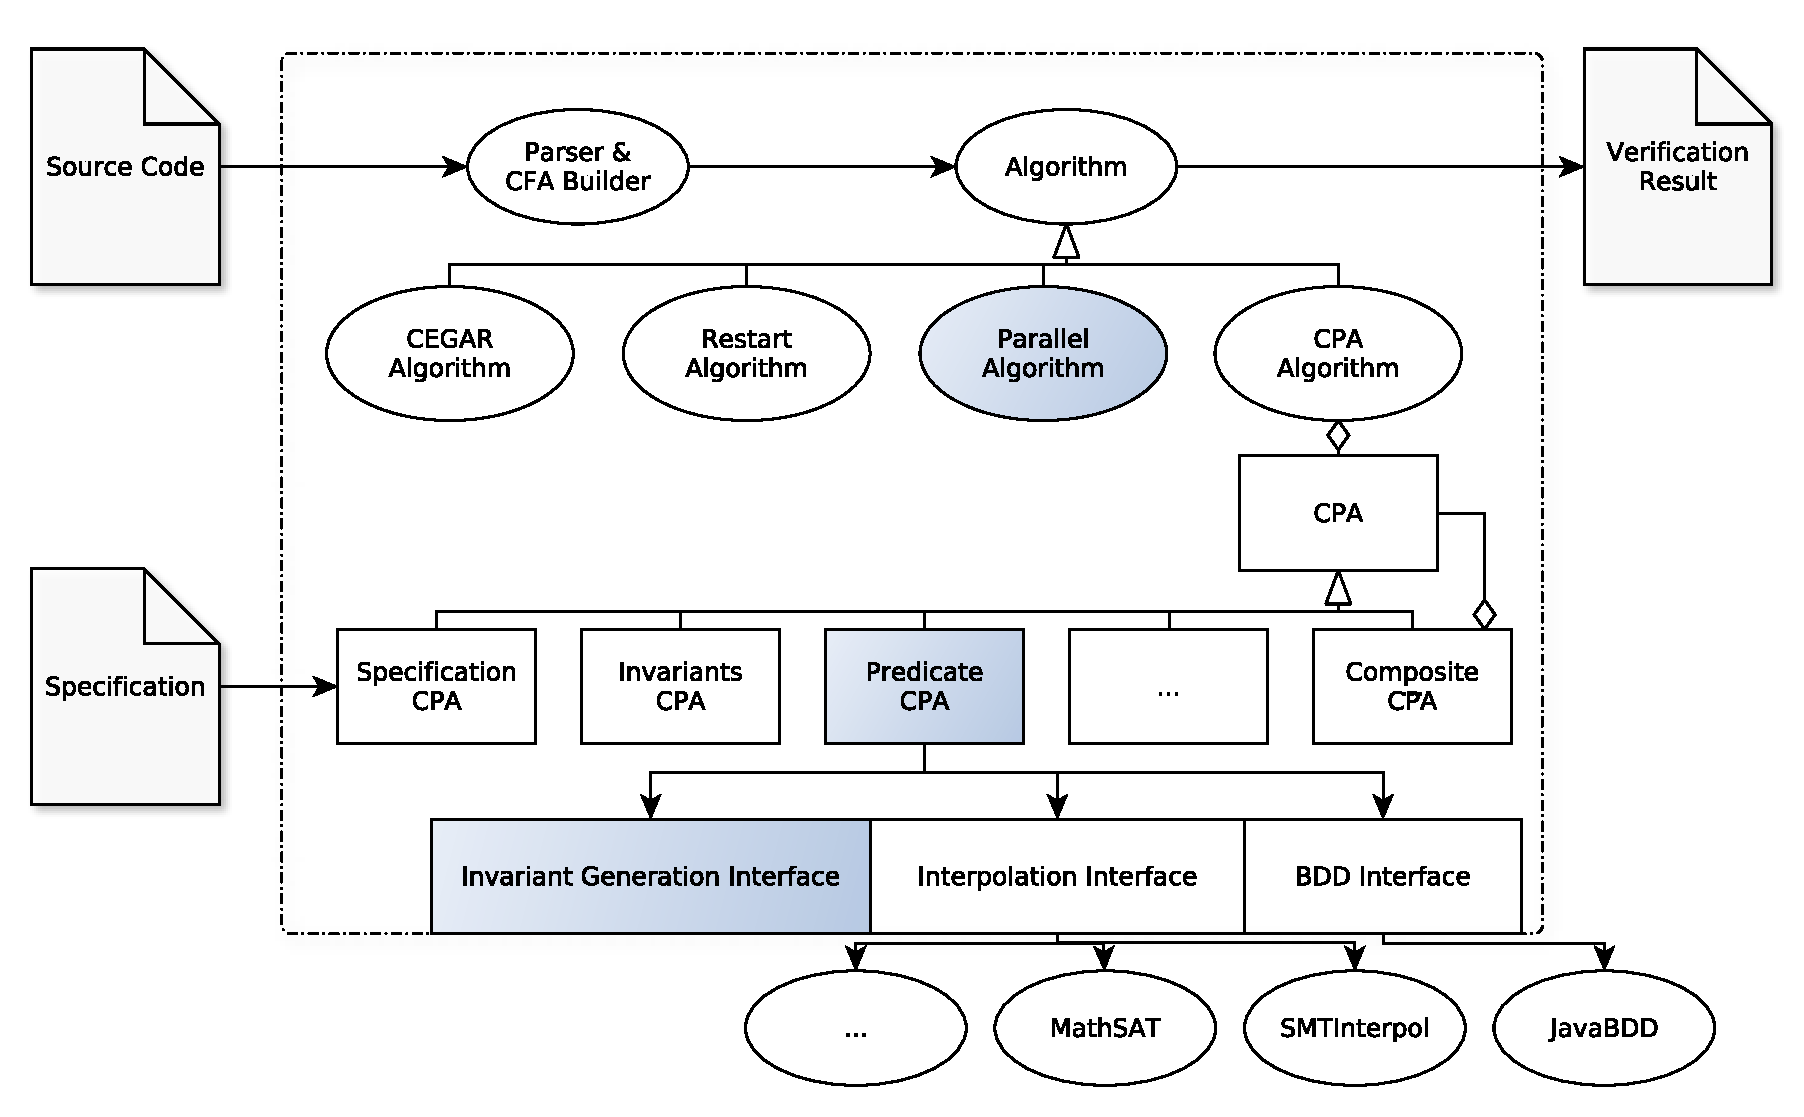
\includegraphics[width=\textwidth]{../graphics/CPAchecker_architecture}
 \caption{\CPAchecker{} architecture~\cite{Beyer:CPAchecker}}
 \label{fig:CPAchecker_architecture}
\end{figure}

\subsection{Basic Architecture}
In \autoref{fig:CPAchecker_architecture} the basic \CPAchecker{} architecture is shown. The highlighted parts are especially important for this thesis, for example the Parallel Algorithm is even added in this thesis, but already in the figure to show where it is located compared to other \CPAchecker{} components.

A simple verification run could work as follows: at first the source code is parsed\,\sidenote{We use the Eclipse CDT for that purpose, it can be found at \url{eclipse.org/cdt/}}, then a \ac{CFA} is created and afterwards the result is computed by the $\CPAAlgorithm{}$ with the configured \acp{CPA}. The result is then given to the user of \CPAchecker{}.

\subsection{Composite CPAs in \CPAchecker{}}
The concept of a composite analysis, introduced in \autoref{title:compositeCPA}, 
enables us to separate the different concerns of component analyses from each other. The component \acp{CPA} can then be combined on demand. Two important features for every analysis are tracking the call-stack and the program counter. So, instead of repeatedly implementing tracking of the location and the call-stack for every analysis, one can now create separate \acp{CPA} for modeling the call-stack and tracking the program counter.

\subsection{Sequential Combination of Analyses}\label{title:restart}
Sequentially combining several separate analyses is a concrete implementation of conditional model checking~\cite{Beyer:ConditionalModelChecking} (cf. \autoref{title:cmc}).
This approach is also implemented in \CPAchecker{} in the $\mathtt{RestartAlgorithm}$. Whenever the result of a verification run is not \emph{safe} or \emph{unsafe}, the next configuration is started with the input condition \false{} and has to verify the program without any initial assumptions again. Furthermore it is possible to skip subsequential analyses based on the outcome of earlier ones, for example if an analysis finds out that the program contains concurrency, all analyses which do not support concurrency can be omitted, prohibiting the model checker from consuming time with analyses that do not provide the necessary abilities.


\subsection{Counterexample-Guided Abstraction Refinement}\label{title:cegar}
\AC{CEGAR}~\cite{Clarke:CEGAR} is a technique that tries to overcome the state space explosion in model checking by abstracting unnecessary information. This is done by iteratively refining the precision of the analysis each time an infeasible counterexample is identified. The necessary information for refining the precision can be extracted by several techniques out of the infeasible counterexample. Some possibilities are for example Craig interpolation~\cite{Beyer:CPAchecker}, path invariants (cf. \autoref{background:pathinvariants}) or heuristics that extract the precision increment from program statements, \eg, assumptions.

While the original approach is only aimed at symbolic model checking, \ac{CEGAR} has been extended to also work with explicit-state model checkers~\cite{Beyer:ExplicitCEGAR}.


\begin{algorithm}[t]
\LinesNumbered
 \SetKw{Var}{Variables}
 \SetKwInput{Kw}{Variables}
 \KwIn{CPA with dynamic precision adjustment $\mathbb{D} = (D, \precision, \transabs, \mergeop, \stopop, \precop)$, \newline an initial abstract state $e_0 \in E$ with precision $\pi_0 \in \precision$, where $E$ denotes the set of elements of the semi-lattice of~$D$}
 \KwOut{verification result safe or unsafe}
 \Kw{set $\reached \subseteq E \times \precision$, set $\waitlist \subseteq E \times \precision$,  error~path~$\sigma~=~\langle(op_1, l_1),...,(op_n, l_n)\rangle$}
 \BlankLine
 $\reached := \{(e_0, \pi_0)\}$\;
 $\waitlist := \{(e_0, \pi_0)\}$\;
 \While{\true{}}{
  $(\reached, \waitlist) := \CPAAlgorithm(\DD, \reached, \waitlist)$\;
  \eIf{$\waitlist = \emptyset$}{
    \Return{$safe$}
  }{
    $\sigma := \mathsf{extractErrorPath(reached)}$\;
    \BlankLine
    \emph{feasible error: report bug, else refine and restart}\;
    \eIf {$\mathsf{isFeasible}(\sigma)$}{
      \Return{$unsafe$}
     }{
      $\pi := \pi \bigcup \mathsf{refine}(\sigma)$ \;
      $\reached := (e_0, \pi)$\;
      $\waitlist := (e_0, \pi)$\;
    }
  }
 }
 \caption{$\CEGARAlgorithm(\DD, e_0, \pi_0)$~\cite{Beyer:ExplicitCEGAR}}
 \label{alg:CEGAR}
\end{algorithm}

In \autoref{alg:CEGAR} a simple \ac{CEGAR} algorithm working in 
combination with a \ac{CPA} is displayed. The method $\mathtt{extractErrorPath}$
extracts the found counterexample out of the set $\reached$. The feasibility
of the counterexample is tested with the method $\mathtt{isFeasible}$. If the
counterexample is feasible we can stop the analysis and return the found property
violation to the user. When the counterexample is infeasible we use the
procedure $\mathtt{refine}$ to refine the precision of the analysis.

The \ac{CEGAR} algorithm is implemented in \CPAchecker{}, and further more has an additional option which delays the 
refinement until the state space is fully explored with the 
current precision. When this happens the refinement starts and all 
error locations are handled at once. The latter approach will be 
used later on for invariant generation.

\clearpage


\subsection{The \PredicateCPA{}}\label{title:predicatecpa}
The \PredicateCPA{}~\cite{Beyer:PredicateAbstraction} is based on (boolean) predicate abstraction\,\sidenote{While other abstraction methods, such as cartesian
abstraction, are also possible, the default abstraction method is boolean predicate 
abstraction.}. Let $\mathcal{P}$
be a set of predicates over program variables, a formula~$\phi$ is 
a boolean combination of predicates from $\mathcal{P}$. We call $
\pi$ a precision for formulas with $\pi \subset \mathcal{P}$. $
\Pi$ is a precision for programs given by the function $\Pi: L 
\rightarrow 2^\mathcal{P}$, which assigns a precision for formulas 
to each program location. The strongest boolean combination of 
predicates from precision $\pi$ entailed by $\phi$ is called 
boolean predicate abstraction $(\phi)^\pi$ of a formula $\phi$.
The outcome of a predicate abstraction can be used as abstract 
state and represents a region of concrete program states. The 
computation of the predicate abstraction can be done by \ac{SMT} 
solvers. Therefore we introduce a propositional variable 
$v_i$ for each predicate $p_i \in \pi$ and 
then ask the \ac{SMT} solver for satisfying assignments for the formula $\phi \land 
\bigwedge_{p_i \in \pi}(p_i \iff v_i)$. The disjunction of all 
conjuncted satisfying assignments is the result of the boolean 
predicate abstraction. Computing the successor $\phi'$ of $\phi$ is done by applying the abstract
strongest post operator for predicate abstraction with a program operation $op$. The strongest
post operator can be defined as $\phi' = (\mathtt{SP}_{op}(\phi))^\pi$, where $\mathtt{SP}$ denotes
the strongest post condition operator, which is applied first, afterwards, the result is used for
computing the boolean predicate abstraction.

The original predicate abstraction~\cite{Beyer:PredicateAbstraction} works either with \ac{SBE} or with
\ac{LBE} and while \ac{SBE} leads to a slower analysis, we need to preprocess the analyzed program for
\ac{LBE}. Both approaches are unified in \ac{ABE}, an approach which choses dynamically whether an abstraction
should be computed~\cite{Beyer:PredicateAbstraction}. For adding this as a feature to the traditional
predicate abstraction, we store two separate formulas in each state, an abstraction formula $\psi$ and a
path formula $\phi$. States at which an abstraction is done are called \emph{abstraction states}, all other
states are called \emph{non-abstraction states}. Both are disjunct types of abstract states of this \ac{CPA}.
Program paths between two abstraction computations may consist of many \ac{CFA} edges where states for
locations inside such paths are always non-abstraction states. For these non-abstraction states the strongest
post condition is stored in the path formula of each state, while the abstraction formula remains unchanged.
At abstraction states, a new abstraction formula is computed. The decision when to do abstraction is done by
the block-adjustment operator $\blk{}$ which returns \false{} if no abstraction should be computed for a given
pair of an abstract state $e$ and a \ac{CFA} location $l$, and \true{} otherwise. 

By adjusting the block size on demand, we can have many concrete configurations lying in between \ac{SBE} and
\ac{LBE} and even block sizes larger than those produced with \ac{LBE} are possible.
The \PredicateCPA{} with \ac{ABE} is defined as follows\,\sidenote{Please note that the location is not modeled
within this CPA but is still needed, so having a composite with a \ac{CPA} for location tracking is necessary.}:

\begin{itemize}
\item The abstract domain $D_{\mathbb{P}} = (C, \mathcal{E}, \sem{\cdot})$ is given by the semi-lattice $\mathcal{E} = (2^\pi, \text{\true{}}, \text{\false{}}, \sqsubseteq, \sqcup)$, where the partial order $\sqsubseteq \subseteq E \times E$ is defined as
$e_1 \sqsubseteq e_2 \iff (e_2 = T) \lor (\psi_1 \land \phi_1 \Rightarrow \psi_2 \land \phi_2)$ and the join operator $\sqcup: E \times E \rightarrow E$ is defined as the least upper bound of both operands, according to the partial order. The concretization function is given by $\sem{e} = \{c \in C \;|\; c \models \phi_e\}$.

\item The set $\Pi$ of precisions contains the predicates used for predicate abstraction. It is initially empty, and combined with \ac{CEGAR} upon finding infeasible errors, we compute the necessary precision increment to refute the infeasible counterexample using Craig interpolation~\cite{Craig:Interpolation}.

\item The transfer relation  $\transabs \subseteq E \times G \times E \times \precision$ computes the abstract successor $e' = (\psi', \phi')$ for an abstract state $e = (\psi, \phi)$ and a \ac{CFA} edge $g = (l, op, l')$ such that
$\phi' = \mathtt{SP}_{op}(\phi) \land (\psi' = \psi)$ holds.

\item The merge operator $\mergeop : E \times E \times \precision \rightarrow E$ is defined as follows for two states $e_1 = (\psi_1, \phi_1)$ and $e_2 = (\psi_2, \phi_2)$:
\begin{displaymath}
\begin{cases}
e_2 & \text{if this is an abstraction location}\\
e_2 & \text{if } \psi_1 \neq \psi_2 \\
(\psi_1, \phi_1 \lor \phi_2) & \text{otherwise}
\end{cases}
\end{displaymath}

\item The stop operator is $\stopop^{sep}$.

\item The precision adjustment function $\precop : E \times \precision \times 2^{E\times \precision} \rightarrow E \times \precision$ creates for a given abstract state $e$ with precision $\pi$ and a given set of abstract states with precisions a new abstract state $\hat{e}$ with precision $\hat{\pi}$ depending on $\blk{}$. The program location $l$, which is necessary for $\blk{}$, can be retrieved from another CPA that tracks the location and is part of the composite analysis. While the computed abstract state $\hat{e}$ may be different to $e$, the precision stays the same:
\begin{displaymath}
\begin{cases}
\hat{e} = ((\mathtt{SP}_{op}(\phi \land \psi))^{\pi}, \text{\true{}}) & \text{if } \blk{}(e, l)\\
\hat{e} = e & \text{otherwise}
\end{cases}
\end{displaymath}

\end{itemize}

\subsection{The \InvariantsCPA{}}
In contrast to the \PredicateCPA{}, the \InvariantsCPA{}~\cite{Beyer:InvariantsCPA} does not use \ac{SMT} solvers, but is based on expressions over intervals. The important parts of this CPA will be introduced in the following paragraph:

\begin{itemize}
\item The abstract domain of the \InvariantsCPA{} is based on expressions over intervals. Abstract states in this domain are mappings $M: X \rightarrow Expr$ from a set of program variables $X$ to a set of arithmetic expressions $Expr$, where $Expr$ can consist of unary and binary expressions $U = \{\neg,\,\sim,\,-\}$ and $B = \{+,\,*,\,/,\,\%,\,=,\,<,\,\hat{},\,|,\,\lor,\,\&,\,\land,\,\gg,\,\ll,\,\cup\}$, as well as program variables or disjunctions of intervals $I$ of the form $[u, l]$ with $u, l \in \mathbb{Z} \cup \infty$. The (recursive) definition is $Expr \subseteq ((Expr \times B \times Expr) \cup (U \times Expr) \cup X \cup I)$.

\item The set of precisions $\Pi$ contains precisions $\pi = (Y, n, w)$ with $Y \subseteq X$, a maximal expression nesting depth $n \in \mathbb{N}$
and a boolean flag $w \in \mathbb{B}$ specifying whether widening should be used. All abstract states have the same precision. In general, the \InvariantsCPA{}
is tracking all program variables, but most of them are over-approximated while joining states. $Y$ is a selection of important program variables, which are not
over-approximated while joining states. $n$ specifies the accuracy of inter-variable relations. With $w$
set to \true{} widening is used to sacrifice accuracy for efficiency. This is especially important for programs with many loop iterations.

\item The merge operator $\mergeop : E \times E \times \precision \rightarrow E$ is defined as following for two states $e_1$ and $e_2$:
\begin{displaymath}
\begin{cases}
\mathtt{widen}(e_1, e_2) & \text{if } w \land \neg \mathtt{differ}_\pi(e_1, e_2)\\
\mathtt{union}(e_1, e_2) & \text{if } \neg w \land \neg \mathtt{differ}_\pi(e_1, e_2)\\
e_2 & \text{otherwise}
\end{cases}
\end{displaymath}
$\mathtt{differ}$ is a function that checks if the expressions over the important variables $Y$ are equal in both states, if not, we do not merge at all.
A widening is done according to $w$, where widening means that for each variable only a single (potentially infinite) interval is assigned. $\mathtt{union}$
is the union of all values for each variable.
\end{itemize}

While the precision is fixed for a complete verification run it can be configured to be continuously-refined by using \autoref{alg:continously-refined}
as a wrapper around \autoref{alg:cpa}. With this wrapper algorithm, only safe programs can be found, for all other programs, the result will be
unknown\,\sidenote{Due to the fixed precision we do not know if a bug was found because of being to coarse or because the bug actually exists.}.
For example, the first iteration of doing an analysis with the \InvariantsCPA{} is done with an empty set of important variables $Y$, and an expression
nesting depth $n$ of $1$. With each iteration we can now increase $n$ as well as inserting variables into $Y$. If at some time, no state violating the specification
is in the reached set (indicated by the method $\mathtt{containsTargetState}$) \autoref{alg:continously-refined} terminates and tells the user that the program is safe.

An additional feature of \autoref{alg:continously-refined} is that one can extract invariants from it. This is for example
necessary for $k$-induction-based analyses (cf. \autoref{title:kind}). $\mathtt{getCurrentlyKnownInvariants}$ is the name of the corresponding function.

\SetKwFor{Loop}{Loop}{}{EndLoop}
\begin{algorithm}
\LinesNumbered
\SetKw{Var}{Variables}
 \SetKwInput{Kw}{Variables}
 \KwIn{a configurable program analysis with dynamic precision adjustment $\mathbb{D} = (D, \precision, \transabs, \mergeop, \stopop, \precop)$,\newline
       a set of initial abstract states $E$,\newline
       an initial precision $\pi_0$}
 \KwOut{\true{} if no target state is found}
 \Kw{a set $\reached$ of elements of $E \times \precision$,\newline a precision $\pi$,\newline an invariant $Inv$}
   $\pi := \pi_0$\;
   $Inv: = \text{\true{}}$\;
   \Loop{}{
     $\reached := \CPAAlgorithm(\mathbb{D}, \{(e, \pi) | e \in E\}, \{(e, \pi) | e \in E\})$\;
     \If{$\neg \mathtt{containsTargetState}(\reached)$}{
     	\Return{\true{}}
     }
     $Inv := Inv \land \underset{s \in reached}{\bigvee} s$\;
     $\pi := \mathtt{RefinePrec}(\pi)$\;
   }

 \caption{Continuous Precision Refinement and Invariant Generation~\cite{Beyer:InvariantsCPA}}
 \label{alg:continously-refined}
\end{algorithm}